% *********************************************************
% Check "thesis-style.sty" to customise language and others
% *********************************************************

\documentclass[a4paper,12pt,twoside]{ThesisStyle}
\usepackage{thesis-style}
\usepackage[utf8]{inputenc}
\usepackage{enumitem}

\newcommand{\titlemark}{Desenvolupament d’una aplicació òbil de codi obert per a fer pagaments entre usuaris mitjaçant codis QR} % Project title for custom header
\newcommand{\documentmark}{Memòria} % Document type for custom header
\newcommand{\appendixmark}{Annex} % Appendix mark for custom header

% \cftsetindents{section}{1em}{3em}
% \setlength\cftsectionnumwidth{4em} % uncomment to see difference

\begin{document}

\frontmatter

\pagenumbering{gobble}

\thispagestyle{empty}
\begin{table}[htb]
\centering
\begin{Large}
\resizebox{\textwidth}{!}{\begin{tabular}{ | l |}
 \hline
 \\

\includegraphics[scale=0.9]{imatges/logo_eps.png} \\[0.7cm]
\centerline{Projecte fi de grau}\\[1cm]
\hline
\\
Estudi: Grau en Enginyeria Informàtica\\[0.7cm]
\hline
\\
Títol: Desenvolupament d'una aplicació mòbil de codi obert per a fer pagaments\\
entre usuaris mitjaçant codis QR\\[0.7cm]
\hline
\\
Document: Memòria\\[0.7cm]
\hline
\\
Alumne: Sudan Wu\\[0.7cm]
\hline
\\
Tutor: Pau Xiberta i Armengol\\
Departament: INFORMÀTICA, MATEMÀTICA APLICADA I ESTADÍSTICA\\
Àrea: LLENGUATGES I SISTEMES INFORMÀTICS\\[0.7cm]
\hline
\\
Convocatòria (Setembre/2024): XXX\\[0.7cm]
\hline

\end{tabular}}
\end{Large}
\end{table}

\newpage

\begin{titlepage}

% Upper part of the page

\includegraphics[scale=0.9]{imatges/logo_eps.png} \\[1cm]
\begin{center}
\textsc{\Large Projecte Fi de Grau} \\[1cm]

% Title
\begin{spacing}{2}
\HRule \\
\textbf{\Huge Títol del projecte} \\
\HRule \\[0.5cm]
\end{spacing}

% Author and supervisor and other data
{
\large
\emph{Autor:} \\
Nom \textsc{Sudan Wu} \\[1cm]
Setembre 2024 \\[1cm]
Grau en Enginyeria Informàtica \\[1cm]
\emph{Tutor:} \\
Nom \textsc{Pau Xiberta i Armengol} \\
}

\end{center}
\end{titlepage}

\titlepage

\dominitoc

\pagenumbering{roman}

\chapter*{Resum}
\label{chp:resum}



\chapter*{Agraïments}
\label{chp:agraiments}

Per començar vull agrair molt especialment a al meu tutor Pau Xiberta i Armengol, per la seva guia, paciència i saviesa durant tot el procés. Les seves orientacions han estat fonamentals per a la consecució d’aquest treball, i la seva dedicació ha estat una font constant de motivació.\\

També voldria agrair als meus companys i amics per estar sempre al meu costat, oferint suport emocional i consells valuosos en moments de dubte i incertesa. La vostra companyia ha fet aquest viatge molt més suportable i enriquidor.\\

No puc oblidar la meva família, que ha estat el meu pilar més ferm al llarg de tota aquesta etapa acadèmica. Gràcies per creure en mi, per la vostra paciència infinita i per animar-me a seguir endavant, fins i tot en els moments més difícils.\\

Finalment, vull reconèixer l’esforç i dedicació de tots els professors que m’han format durant aquests anys. Les vostres ensenyances han estat fonamentals per arribar fins aquí, i cada una de les vostres lliçons ha deixat una petjada en aquest treball.\\

A tots, gràcies de tot cor per fer possible aquest assoliment.


\tableofcontents

\listoffigures

\listoftables

\mainmatter



\chapter{Introducció, motivació, finalitat i objectius del projecte}
\label{chp:intro}

\section{Introducció}
\label{sec:Introduccio}

A l'hora de processar un pagament, la majoria de botigues utilitzen un Terminal Punt de Venda (TPV) físic, i els clients fan servir una targeta bancària o una cartera digital que incorpora aquesta targeta. El TPV actua com a intermediari en l'operació, introduint un procés addicional que pot augmentar tant els costos com el risc d'errors. Tot i que existeixen plataformes de pagament en línia, aquestes no estan dissenyades per substituir completament el TPV físic, i sovint no són de codi obert ni ofereixen l'opció de realitzar transaccions mitjançant codis QR.

\section{Motivació}
\label{sec:Motivacio}

L’evolució tecnològica i la digitalització han transformat profundament la manera com les empreses gestionen els seus processos de pagament. Tot i els avenços, el sistema tradicional basat en terminals físics de punt de venda (TPV) encara predomina, arrossegant amb si costos operatius elevats i riscos associats a errors humans i fraus. Aquesta situació, sumada a la creixent adopció de tecnologies de pagament mòbil i l’ús de codis QR en diverses parts del món, posa de manifest la necessitat d’explorar alternatives més eficients, segures i accessibles.\\

Aquest projecte neix de la voluntat d’abordar aquestes limitacions, oferint una solució que pugui substituir o complementar els TPV físics amb una plataforma de pagament en línia de codi obert. Una solució que permeti als comerciants processar transaccions mitjançant codis QR, oferint així una experiència de pagament més ràpida, senzilla i segura tant per a les botigues com per als clients.\\

La motivació principal d’aquest projecte és reduir els costos operatius i minimitzar els riscos associats als sistemes de pagament tradicionals, alhora que es promou la inclusió tecnològica a través d’una eina de codi obert, accessible per a qualsevol empresa o desenvolupador que desitgi implementar-la. Creiem que, mitjançant aquesta iniciativa, podem contribuir a la transformació digital del comerç, afavorint la seva competitivitat i adaptabilitat en un mercat cada cop més globalitzat i dinàmic.

\section{Finalitat i objectius del projecte}
\label{sec:Finalitat i objectius del projecte}

L'objectiu d'aquest treball de final de grau és desenvolupar una aplicació full stack que inclogui totes les funcions necessàries per gestionar pagaments mitjançant codis QR. Aquest desenvolupament inclourà:

\begin{itemize}
  \item El disseny i la implementació de la base de dades per emmagatzemar la informació de les transaccions i els usuaris.
  \item El desenvolupament d'una API que permeti interactuar de manera eficient amb la base de dades, facilitant la creació, gestió i consulta de pagaments.
  \item La creació d'una interfície d'usuari senzilla i intuïtiva, que permeti als usuaris generar i escanejar codis QR per realitzar transaccions.
  \item El desenvolupament de les aplicacions frontals basades en aplicacions que permetin als usuaris accedir al sistema, generar codis QR i realitzar els pagaments de manera segura i ràpida.
\end{itemize}

L'aplicació permetrà als clients generar codis QR tant per realitzar pagaments com per rebre cobraments, que podran ser escanejats amb qualsevol dispositiu que tingui càmera per completar la transacció.


\chapter{Viabilitats}
\label{chp:viabilitats}

\section{Introducció}
\label{subsec: Introducció}

L'estudi de la viabilitat del projecte es tindrà en compte des de la tècnica
recursos, cost econòmic del projecte i viabilitat del mercat.\\

En conjunt demostra que el projecte és viable i té un alt potencial de creixement en l'entorn actual, oferint una solució innovadora i segura per als pagaments mòbils a través de codis QR.

\section{Viabilitat tècnica}
\label{subsec:Viabilitat tècnica}

L'aplicació utilitzarà Node.js i apollo server per a la gestió del servidor i Flutter per al desenvolupament de la interfície d'usuari. A més, es farà servir una base de dades en MongoBD per emmagatzemar les transaccions i informació dels usuaris. Aquestes tecnologies són àmpliament utilitzades i ben suportades per la comunitat de desenvolupadors.

\section{Viabilitat econòmica}
\label{subsec:Viabilitat económica}

Els costos principals del projecte inclouen el desenvolupament de l'aplicació, que es realitzarà internament, i els costos d'allotjament en el núvol, que seran proporcionats per serveis com AWS amb un pressupost de X euros mensuals.\\

El sistema de pagament mitjançant codis QR ofereix una solució econòmica en comparació amb els terminals de TPV tradicionals, amb una possible font d'ingressos a través de comissions per transacció i opcions de subscripció per serveis addicionals.



\section{Viabilitat de mercat}
\label{subsec:Viabilitat de mercat}

Amb l'augment de l'ús de pagaments mòbils i la necessitat de solucions de pagament contactless, hi ha una demanda creixent per a sistemes de pagament basats en codis QR. Aquesta tendència proporciona una oportunitat significativa per a la nostra aplicació.

Encara que hi ha altres solucions de pagament basades en codis QR, el nostre sistema es diferencia per la seva integració fàcil amb altres plataformes i la seva estructura de codi obert, que permet personalització i adaptació a les necessitats específiques dels usuaris.


\chapter{Metodologia}
\label{chp:metodologia}


\section{Introducció}
\label{subsec: Introducció}

La metodologia utilitzada en aquest projecte és àgil Scrum, tot i que es tractava d'un projecte individual. 

\section{Scrum}
\label{subsec: Scrum}

Scrum és un marc de treball per a la gestió de projectes, conegut per la seva flexibilitat i per permetre gestionar projectes complexos a través de cicles iteratius de treball anomenats sprints. Encara que tradicionalment Scrum està dissenyat per a equips, es van adaptar els seus principis per optimitzar la gestió del temps i els recursos durant el desenvolupament del projecte.\\

\begin{figure}[h!] % La posició de la figura pot ser ajustada amb 'h!', 't', 'b', etc.
  \centering
  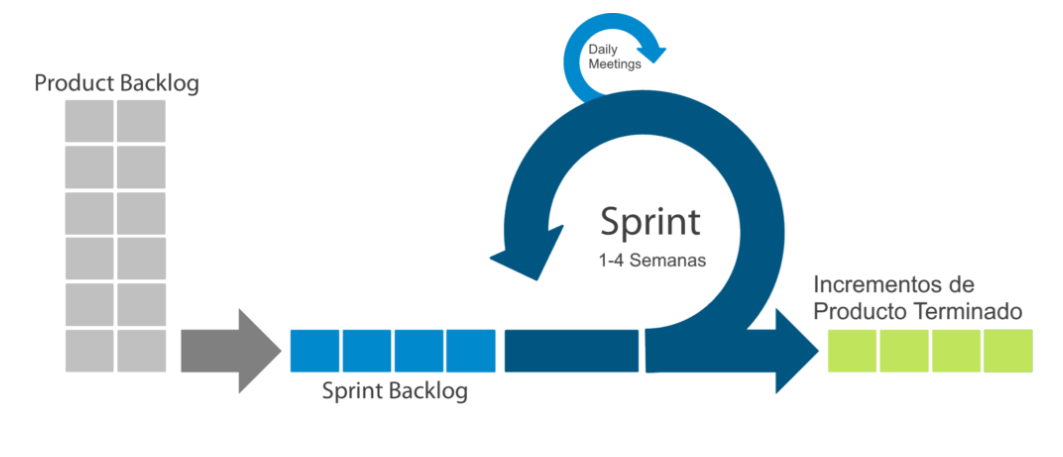
\includegraphics[width=0.8\textwidth]{imatges/scrum.png} % Ajusta el nom i el camí del fitxer d'imatge
  \caption{Sistema de treball Scrum} % Títol de la imatge
  \label{fig:exemple} % Etiqueta per referenciar la imatge
\end{figure}

L'elecció de Scrum es va basar en la necessitat de mantenir una alta capacitat de resposta davant els canvis en els requisits i per estructurar el procés de desenvolupament en fases manejables. Scrum va permetre dividir el projecte en sprints, cosa que va facilitar la planificació i el seguiment del progrés, assegurant-se que cada fase del projecte es completava abans de passar a la següent.\\

Per a la planificació del projecte, es defineixen sprints de dues setmanes, cadascun amb objectius específics que cal complir abans d’iniciar el següent sprint. Al principi de cada sprint, s’elabora un pla detallat de les tasques a realitzar, prioritzant les més crítiques i assegurant que estan alineades amb els objectius generals del projecte.\\

Es crea i es gestiona un product backlog que llista totes les funcionalitats a desenvolupar. Aquest backlog es prioritza d’acord amb la seva importància i la complexitat de la implementació. Cada sprint es planifica tenint en compte aquesta llista, garantint que es treballa sempre en les tasques més rellevants per al progrés del projecte.\\

L'ús de Scrum, adaptat a un entorn individual, va ser fonamental per a la gestió eficient del temps i la consecució dels objectius del projecte. Va permetre que el desenvolupament es realitzés de manera ordenada i progressiva, proporcionant la flexibilitat necessària per fer ajustos sobre la marxa. Aquesta metodologia va resultar especialment útil per mantenir el ritme de treball i assegurar que cada fase del projecte es completés amb èxit abans de passar a la següent.



\chapter{Planificació}
\label{chp:planificació}

\section{Introducció}
\label{sec:Introducció}

El següent pla de planificació ofereix una visió clara del procés de desenvolupament del projecte, destacant les etapes clau, el temps assignat i els resultats esperats, així com l'aplicació de la metodologia Scrum per gestionar el projecte de manera àgil.



\section{Desenvolupament}

El procés de creació i construcció del producte de programari inclou les següents tasques:

\begin{enumerate}
  \item \textbf{Anàlisi de Requisits}:
  \begin{itemize}
      \item Revisar els requisits del projecte.
      \item Establir especificacions detallades per al desenvolupament.
  \end{itemize}

  \item \textbf{Disseny}:
  \begin{itemize}
      \item Crear l'arquitectura del sistema.
      \item Dissenyar les interfícies d'usuari i les interaccions.
      \item Definir les estructures de dades i les lògiques d'operació.
  \end{itemize}

  \item \textbf{Codificació}:
  \begin{itemize}
      \item Escriure el codi font segons les especificacions.
      \item Implementar les funcionalitats del sistema.
      \item Desenvolupar codi de backend amb Apollo-server i frontend amb Flutter
  \end{itemize}

  \item \textbf{Integració}:
  \begin{itemize}
      \item Combinar diversos mòduls o components.
      \item Assegurar que els components funcionin conjuntament.
  \end{itemize}

  \item \textbf{Proves}:
  \begin{itemize}
      \item Crear i executar proves per verificar la funcionalitat de cada component.
      \item Corregir errors detectats durant les proves.
  \end{itemize}

  \item \textbf{Revisió de Codi}:
  \begin{itemize}
      \item Realitzar revisions de codi per assegurar la qualitat i el compliment dels estàndards.
  \end{itemize}

  \item \textbf{Documentació}:
  \begin{itemize}
      \item Elaborar memòria sobre l’arquitectura, el disseny i el codi.
  \end{itemize}

  \item \textbf{Manteniment i Actualitzacions}
    \begin{itemize}
        \item Realitzar manteniment regular del sistema per assegurar la seva funcionalitat.
        \item Implementar actualitzacions i millores basades en feedback i nous requisits.
    \end{itemize}


\end{enumerate}


\subsection{Calendari previst}
\label{subsec: Calendari previst}

\begin{table}[h!]
\centering
\begin{tabular}{|c|c|c|c|c|}
\hline
\textbf{Núm.} & \textbf{Fase} & \textbf{Data d'Inici} & \textbf{Data de Finalització} & \textbf{Resultats}\\
\hline
1 & Anàlisi de Requisits & 01/04/2024 & 07/04/2024 & ok \\
2 & Disseny & 08/04/2024 & 21/04/2024 & ok\\
3 & Codificació & 22/04/2024 & 15/06/2024 & ok\\
4 & Integració & 16/06/2024 & 30/06/2024 & ok\\
5 & Proves & 01/07/2024 & 15/07/2024 & ok\\
6 & Revisió de Codi & 16/07/2024 & 31/07/2024 & ok\\
7 & Documentació & 1/08/2024 & 31/08/2024 & ok\\
8 & Manteniment i Actualitzacions & 01/09/2024 & Continu & ok\\
\hline
\end{tabular}
\caption{Calendari del projecte}
\label{tab:calendari}
\end{table}



\chapter{Marc de treball i conceptes previ}
\label{chp:marcdetreball}


\section{Introducció}
\label{subsec:Introducció}

En aquest capítol es tractaran els coneixements necessaris per desenvolupar correctament una aplicació bancària que utilitza codi QR per realitzar operacions. En resum, és important entendre com funciona el codi QR, especialment en relació amb com emmagatzemar el contingut. A més, cal disposar de coneixements sobre arquitectura i desenvolupament de programari per aportar valor a l'aplicació.

\subsection{Propòsit}
\label{subsubsec: Propòsit}

L'objectiu de l'aplicació és proporcionar una plataforma senzilla, escalable i potent per gestionar els pagaments i cobraments mitjançant codi QR. Tant els clients com els comerciants tindran accés a les mateixes funcionalitats i permisos dins de l'aplicació. Els comerciants podran configurar els seus sistemes de pagament, establir les opcions disponibles, ajustar els límits de transacció i altres configuracions relacionades. D'altra banda, els clients podran realitzar pagaments i cobraments a través de codis QR amb facilitat. A més de facilitar les compres, l'aplicació permetrà als usuaris realitzar transferències entre amics i familiars, oferint una solució versàtil per diverses necessitats financeres quotidianes.


Per tant, en una sola aplicació, els comerciants podran controlar totes les transaccions que es realitzin, alhora que tindran la capacitat d'aplicar canvis i modificacions segons les seves necessitats i preferències.



\begin{itemize}
  \item User: L'usuari es la persona principal que utiliza l'aplicació. En aquest cas, ho es el administrador i els seus clients.
\end{itemize}



\chapter{Requisits del sistema}
\label{chp:requisits}

En aquesta secció, s'explicaran amb més profunditat els requisits descrits anteriorment.
Els requisits funcionals es defineixen com les funcionalitats bàsiques del sistema.
Tots els requisits exposats a la secció es consideren essencials i del sistema
es consideraria incompleta si no complia aquests requisits.






\section{Introducció}
\label{subsec:Introducció}

Aquest capítol tractarà l'especificació de requisits del sistema (SRS) per al programari que s'està desenvolupant. L'objectiu d'aquest capítol és establir les bases del que es desenvoluparà, tenint en compte les necessitats dels usuaris, així com els requisits funcionals i no funcionals.


\subsection{Els requeriments funcionals i les novetats d'aplicació}
\label{subsec:Els requeriments funcionals i les novetats d'aplicació}


La funcionalitat bàsica de la meva aplicació és fer transferencies de diners entre 2 usuaris, 
seria una funció de tipu "Bizum", però incorporant el servei de pagament/cobrament mitjançant codi QR. El Bizum està vinculat a un número de telèfon, mentre que en la meva aplicació es vincularà a un número de compte bancari. Cada compte bancari serà capaç de generar codis QR per a cobraments o, a la inversa, serà capaç de llegir codis QR per a efectuar pagaments.\\



\textbf{Gestió d'Usuaris:}
\begin{itemize}
    \item \textbf{RF-1.} Els usuaris client han de poder registrar amb informació bàsica.
    \item \textbf{RF-2.} Els usuaris client/administrador han de poder iniciar sessió a l'aplicació utilitzant les seves credencials.
    \item \textbf{RF-3.} Els usuaris han de poder modificar contrasenya d'accés. No esta feta
\end{itemize}


\textbf{Operacions d'usuari administrador:}
\begin{itemize}
    \item \textbf{RF-4.} Els usuaris administradors han de poder veure tots els usuaris clients i tots els moviments de cadascun.
    \item \textbf{RF-5.} Els usuaris administradors han de poder mantenir clinets(donar alta, donar baixa, eliminar,modificar dades, activat/desactivar funcionalitats...). No esta feta
\end{itemize}


\textbf{Operacions de transaccións d'usuari client:}
\begin{itemize}
    \item \textbf{RF-6.} Els usuaris clients han de poder generar un codi QR únic associat al seu compte per rebre pagaments.
    \item \textbf{RF-7.} Els usuaris clients han de poder escanejar codis QR generats per altres usuaris per fer pagaments/cobraments.
    \item \textbf{RF-8.} Els usuaris han de poder configurar l'import màxim de la transacció mitjançant codi QR.
    \item \textbf{RF-9.} Els usuaris clients han de poder anul·lar la validesa d'un codi QR de pagament. No esta feta
\end{itemize}

\textbf{Funcionalitats addicionals:}
\begin{itemize}
    \item \textbf{RF-10.} La sessió es tanca automàticament en 1 minut si no està en ús. No esta feta
    \item \textbf{RF-11.} Es genera automaticament un comprovant de transacció. No esta feta
    \item \textbf{RF-12.} Els usuaris han de tenir accés a un historial de totes les transaccions realitzades, incloent detalls com ara la data, l'import i l'estat del pagament.
    \item \textbf{RF-13.}L'aplicació ha d'enviar notificacions als usuaris per informar-los sobre l'estat de les seves transaccions, com ara pagaments rebuts o completats.
    \item \textbf{RF-14.} Eines d'informes i anàlisi de dades per als usuaris. No esta feta
\end{itemize}


\textbf{Integracions i Serveis Complementaris:}
\begin{itemize}
        \item \textbf{RF-15.}S'han d'implementar mesures de seguretat robustes, com ara autenticació de dos factors i xifrat de dades, per protegir la informació personal i financera dels usuaris.
\end{itemize}


\subsection{Els requeriments no funcionals i les novetats d'aplicació}
\label{subsec:Els requeriments no funcionals i les novetats d'aplicació}

\textbf{Els requisits no funcional són:}
\begin{itemize}
    \item \textbf{RNF-1.} L'aplicació ha de ser ràpida i eficient, amb temps de càrrega mínims i una resposta àgil a les interaccions de l'usuari.
    \item \textbf{RNF-2.} L'aplicació ha d'estar disponible i accessible en tot moment, amb una infraestructura que garanteixi una alta disponibilitat i temps d'inactivitat mínims.
    \item \textbf{RNF-3.} L'aplicació ha de poder gestionar un alt volum de transaccions i usuaris concurrents, amb la capacitat d'escalar horitzontalment segons sigui necessari.
    \item \textbf{RNF-4.} La interfície d'usuari ha de ser intuitiva i fàcil d'utilitzar, amb un disseny net i clar que permeti als usuaris realitzar les seves tasques de manera eficient.
    \item \textbf{RNF-5.}L'aplicació ha de ser compatible amb una varietat de dispositius i sistemes operatius, incloent telèfons mòbils, tauletes i ordinadors d'escriptori.
    \item \textbf{RNF-6.}S'han d'implementar pràctiques de seguretat sòlides per protegir la integritat i la confidencialitat de les dades dels usuaris, així com per prevenir frau i atacs cibernètics.
\end{itemize}


\subsection{Matriu de dependències de requisits}
\label{Matriu de dependències de requisits}



\chapter{Estudi i decisions}
\label{chp:estudi}


\subsection{Fer estudi sobre protocols d'intercanvi de dades bancàries}

De protocols ens podem dividir en 2 grups: Protocols estàndard (codi obert) i protocols propietaris. Els \textbf{protocols estàndard} es refereixen a un conjunt de regles, especificacions i convencions àmpliament acceptades i utilitzades en una indústria o camp particular. Aquests protocols estan dissenyats per garantir la interoperabilitat, la compatibilitat i la consistència entre diferents sistemes, dispositius o aplicacions que necessiten comunicar-se entre sí. Mentre que els \textbf{protocols propietaris} poden oferir característiques i funcionalitats úniques que diferencien el protocol i proporcionen un valor afegit per als usuaris. \\

\textbf{Protocols estàndards: codi obert}
\begin{itemize}
    \item \textbf{HTTPS} (Hypertext Transfer Protocol Secure): HTTPS és un protocol de transferència de hipertext segur que s'utilitza per a les comunicacions en línia segures, com ara l'accés a portals bancaris en línia i altres serveis financers a través d'Internet. HTTPS encripta les dades durant la transmissió per evitar l'intercepció no autoritzada.
    \item \textbf{FTPs or SFTP:} els protocols de transmissió genèrics utilitzats habitualment en el sector bancari, SSL es pot utilitzar per xifrar les transferències de fitxers, garantint la confidencialitat i la integritat de les dades transferides.
    \item \textbf{SSL: } Secure Sockets Layer és un certificat digital que autentica la identitat d'un lloc web i habilita una connexió xifrada. Un protocol de seguretat que crea un enllaç xifrat entre un servidor web i un navegador web.
\end{itemize}

\vspace{3mm}

\textbf{Protocols propietaris: pagament}
\begin{itemize}
    \item \textbf{FIX} (El protocol d'intercanvi d'informació financera) és un protocol de missatgeria estàndard de la indústria que s'utilitza per a la comunicació electrònica de missatges relacionats amb el comerç entre institucions financeres, com ara bancs d'inversió, corredors i borses de valors.
    \item \textbf{SWIFTNet:} el protocol bancari internacional.
    \item \textbf{EBICS or EBICS TS:} el protocol bancari francès i alemany.
    \item \textbf{PeSit:} el protocol de transmissió genèric per a les institucions regulades franceses
\end{itemize}

\vspace{3mm}

Finalment hi existeix una tercera opció que és crear el \textbf{propi protocol} de seguretat fent servir el xifratge asimetrica. El xifrat asimètric, també conegut com a xifrat de clau pública, és una tècnica criptogràfica que utilitza un par de claus relacionades matemàticament: una clau pública i una clau privada. Aquestes claus estan vinculades de tal manera que la informació xifrada amb una de les claus només pot descifrar-se amb l'altra clau del par.

Algunes algotitmes i tecnologies de la clau asimétrica són:
\begin{itemize}
    \item Diffie-Hellman
    \item RSA
    \item DSA
    \item ElGamal
\end{itemize}

\vspace{5mm}


\subsection{Fer estudi sobre diferents possibilitats per desenvolupar una app i simular un servidor (entorns, llenguatges, etc.)}


\textbf{Alguns dels populars framework de desenvolupament frond-end:}
\begin{itemize}
    \item Flutter (Dart): per ios i Android
    \item React Native (javaScript): per ios i Android 
    \item Ionic:  per ios i Android 
    \item Native Android Development: només per Android
    \item Native ios Development: només per ios
\end{itemize}

\vspace{5mm}

\textbf{Alguns dels populars framework de desenvolupament back-end:}
\begin{itemize}
    \item \textbf{NodeJS:} és un entorn d'execució multiplataforma de codi obert que utilitza JavaScript per al desenvolupament del servidor. Té un conjunt d'eines incorporat que ajuda els desenvolupadors a utilitzar el codi JavaScript per crear aplicacions web i API. Node.js pot crear tot el backend i processar les dades d'aquesta manera, mitjançant la gestió de dades i la gestió dels usuaris.
    \item \textbf{ApolloServer:} és una plataforma de servidor GraphQL de codi obert creada per Apollo GraphQL. És una eina molt popular entre els desenvolupadors per a la creació de servidors GraphQL en entorns de JavaScript, incloent Node.js.
    \item \textbf{Spring Boot: }és un marc popular per crear aplicacions basades en Java, conegut per la seva senzillesa, productivitat i una àmplia gamma de funcions que simplifiquen el procés de desenvolupament. Tanmateix, el desenvolupament de programari és divers i és essencial conèixer les opcions alternatives de Spring Boot que s'adaptin millor als requisits i objectius del vostre projecte.
\end{itemize}



\section{ESCOLLIR ENTORN (DECISIONS)}


\subsection{Escollir un protocol d'intercanvi de dades bancàries}

*Pendent de decidir, segurament un d'estandart*

\subsection{Escollir un entorn i llenguatge per desenvolupar el app i simular un servidor}








\textbf{Triar Frond-end:}

\vspace{3mm}

Destacar Flutter, React i Ionic i fer una comparació, ja que estem tractant amb una aplicació multiplataforma:

    \begin{table}[htbp]
    \centering
    \begin{tabular}{|l|l|l|}
    \hline
    \textbf{Framework} & \textbf{Llenguatge de Programació} & \textbf{Rendiment}                         \\ \hline
    Flutter            & Dart                                                       & Alt                  \\ \hline
    React Native       & JavaScript                                                  & Moderat               \\ \hline
    Ionic              & HTML, CSS, JavaScript                                       & Moderat               \\ \hline
    \end{tabular}
    \end{table}

Les característiques de \textbf{Flutter} són més favorables que les dels altres dos, l'únic inconvenient és que cal aprendre a utilitzar el \textbf{llenguatge Dart}, però no es tracta d'un llenguatge de programació completament desconegut. També té les següents característiques d'avantatge:
\begin{itemize}
    \item\textbf{Widget d'interfície d'usuari personalitzat:} Flutter utilitza un enfocament basat en widgets per construir interfícies d'usuari. Els witgets són blocs de construcció bàsics que es combinen per formar la interfície d'usuari de l'aplicació. Flutter proporciona una àmplia gamma de ginys personalitzables i d'alt rendiment per construir interfícies d'usuari atractives i fluides.
    \item\textbf{Hot Reload:} Una de les característiques més destacades de Flutter és el Hot Reload, que permet veure els canvis a temps real mentre es desenvolupa l'aplicació. Això accelera significativament el procés de desenvolupament en permetre als desenvolupadors fer canvis ràpids i veure els resultats immediatament, sense necessitat de tornar a compilar laplicació.
    \item\textbf{Comunitat activa i creixement:} Flutter compta amb una comunitat activa de desenvolupadors i contribuents que proporcionen suport, recursos d'aprenentatge i paquets de codi obert per facilitar el desenvolupament d'aplicacions. A més, Flutter està experimentant un creixement significatiu i està sent adoptat per una àmplia gamma d'empreses i desenvolupadors a tot el món.
\end{itemize}

\vspace{5mm}

\textbf{Triar Back-end:}

\vspace{3mm}

He escollit el \textbf{apollo server} per següents motius:
\begin{itemize}
    \item Totalment compatible amb GraphQL: Apollo Server és totalment compatible amb totes les especificacions de GraphQL, la qual cosa permet als desenvolupadors crear i exposar una \textbf{API GraphQL} amb facilitat.
    \item Configuració flexible: Apollo Server ofereix una configuració flexible que permet als desenvolupadors personalitzar i adaptar el servidor GraphQL segons les seves necessitats específiques. Això inclou la capacitat de definir tipus de dades, resolvents i esquemes GraphQL de manera eficient.
    \item Integració amb clients GraphQL: Apollo Server s'integra perfectament amb clients GraphQL, com ara Apollo Client, la qual cosa facilita la creació d'aplicacions d'extrem a extrem basades en GraphQL.
    \item Escalabilitat i rendiment: Apollo Server està dissenyat per ser altament escalable i eficient, la qual cosa el fa adequat per manejar grans càrregues de treball i escenaris de trànsit elevat.
    \item Eines i utilitats: Apollo Server proporciona una varietat d'eines i utilitats per facilitar el desenvolupament i la depuració de servidors GraphQL, incloent una interfície gràfica d'usuari (GUI) per explorar l'esquema GraphQL i una consola de depuració interactiva.
\end{itemize}

Els llenguatges de programació específics per al servidor GraphQL són JavaScript o TypeScript. Farè servir el \textbf{Typescript} com llenguatge de programació, perquè TypeScript ofereix diverses avantatges sobre JavaScript, incloent tipat estàtic, millor suport per a eines de desenvolupament, codi més llegible i mantenible, major escalabilitat i compatibilitat amb JavaScript existent. Aquestes avantatges fan que TypeScript sigui una opció atractiva, especialment per a projectes grans i complexos on la qualitat del codi i la mantenibilitat són prioritàries.



\subsection{Escollir un sistema de control de versions i crear repositori de codi obert}

PFG codi: https://github.com/WulinSudan/PFG-code-.git\\
\\
PFG memòria: https://github.com/WulinSudan/PFG.git




\chapter{Anàlisi i disseny del sistema}
\label{chp:analisi}



\chapter{Implementació i proves}
\label{chp:implementacio}



\chapter{Implantació i resultats}
\label{chp:implantacio}

\section{Prova 1}
\section{Prova 2}
\section{Prova 3}
\section{Prova 4}
\section{Prova 5}
\section{Prova 6}
\section{Prova 7}
\section{Prova 8}
\section{Prova 9}
\section{Prova 10}
\section{Prova 11}



\chapter{Conclusions}
\label{chp:conclusions}



\chapter{Treball futur}
\label{chp:treballfutur}

A més, com a funcionalitats futures, tot i que no són prioritàries en aquesta fase inicial del projecte, el sistema també podria incloure:

\begin{itemize}
  \item Una pàgina d'anàlisi que proporcioni informació detallada sobre les transaccions realitzades, ajudant els comerciants a gestionar millor les seves vendes.
  \item Un sistema de subscripcions que permeti als clients realitzar pagaments recurrents de manera automàtica.
\end{itemize}

Aquestes funcionalitats addicionals estan pensades per ampliar les capacitats del sistema i oferir un valor afegit tant als comerciants com als clients, contribuint així a una experiència de pagament més fluida i moderna.

% \backmatter % From this point, chapters are unnumbered


%%%%%%%%%%%%%%%%%%%%%%%%%%%%%%%%%%%%%%%%%%%%
% GETI projects: bibliography as a chapter
%%%%%%%%%%%%%%%%%%%%%%%%%%%%%%%%%%%%%%%%%%%%
%\chapter{Bibliografia}
%\renewcommand{\bibsection}{} % Remove intrinsic bibliography name

\bibliographystyle{ThesisStyleBreakable}
\bibliography{bibliography}

%%%%%%%%%%%%%%%%%%%%%%%%%%%%%%%%%%%%%%%%%%%%
% GETI projects: move "\backmatter" after bibliography to allow unnumbered appendices
%%%%%%%%%%%%%%%%%%%%%%%%%%%%%%%%%%%%%%%%%%%%
% \backmatter



% APPENDICES

% 1. Short and limited command for appendices:
% \appendix

% 2. Full command for appendices (package 'appendices' needed in the preamble: check 'thesis-style.sty'):
% \usepackage[title]{appendix} % add 'titletoc' to add "Appendix" to ToC

% \begin{appendices}

% To manually set appendix chapter names (should be after "\backmatter"):
% \renewcommand{\chaptermark}[1]{\markboth{#1}{}}
% \chapter{Appendix A. Appendix name}

% To let the package manage appendix chapter names (before "\backmatter"):
% \chapter{Appendix name}

% Alternative for separated appendices:
% \include{Appendix1}

% \end{appendices}

% 3. No command for appendices (just unnumbered chapters):
% \renewcommand{\chaptermark}[1]{\markboth{#1}{}}
% \chapter{Appendix A. Appendix name}


%%%%%%%%%%%%%%%%%%%%%%%%%%%%%%%%%%%%%%%%%%%%
% GETI projects: change header to show appendix mark
%%%%%%%%%%%%%%%%%%%%%%%%%%%%%%%%%%%%%%%%%%%%
% \fancyhead[RE,LO]{\bfseries\color{black}\appendixmark}    % Appendix mark (boldface) in the right on even pages, and in the left on odd pages


\renewcommand\appendixname{Annex} % Appendix name (change default)

\begin{appendices}

\chapter{Pressupost}

Lorem ipsum dolor sit amet, consectetur adipiscing elit. Nunc congue mattis tellus, in rhoncus nisl laoreet vel. Sed nulla libero, tincidunt id ligula congue, hendrerit maximus mi. Morbi nec metus in urna imperdiet mattis pretium a libero. Fusce est mauris, convallis id facilisis faucibus, consequat aliquet eros. Vivamus et dui pulvinar, rutrum velit at, volutpat tellus. Nulla vehicula ullamcorper justo, blandit interdum leo sagittis quis. Quisque convallis vel ante ac rutrum. Morbi et varius sem, sed tristique elit. Vestibulum aliquam facilisis pellentesque. Suspendisse consequat commodo eros, sit amet tincidunt sapien semper in. Nunc ut magna ac quam tempor malesuada et at ex. Donec mattis mauris ante, id condimentum elit dapibus at.

Curabitur ut sodales sapien. Etiam eget ultrices risus, in dignissim nunc. Quisque quis tortor in nunc posuere lacinia ut sed dui. Praesent ut sollicitudin diam, ut mattis magna. Morbi porttitor fermentum magna a pharetra. Nullam at magna diam. Suspendisse vehicula tellus eget ligula aliquam semper. Integer sed ullamcorper felis, ac imperdiet elit. Praesent eu suscipit ligula, sit amet vulputate erat. Etiam eget tempor est, vitae aliquet tortor. Nam efficitur tristique ligula. Aliquam blandit leo non ante suscipit, vitae mattis diam rhoncus. Ut ac dui sit amet dui venenatis suscipit.

Nunc sollicitudin hendrerit risus, quis ultricies orci elementum non. Aliquam erat volutpat. Mauris neque turpis, molestie in tellus id, pharetra gravida mi. Suspendisse potenti. Donec aliquam dolor eu pellentesque auctor. Proin eget sapien ut tellus maximus lacinia. Praesent blandit pretium mi, suscipit sollicitudin eros iaculis in. Nunc a justo sit amet mauris auctor posuere sit amet vel erat. Etiam in maximus nisi. Pellentesque blandit pharetra lectus nec efficitur. Praesent tristique vel arcu id bibendum. In eget eros fringilla magna hendrerit facilisis ac vitae urna. Donec malesuada fermentum dictum. Pellentesque aliquet tortor vitae suscipit tempus. Phasellus ornare risus mi, vel placerat justo efficitur eu. Phasellus quis tincidunt enim.

Etiam a elementum lorem. Integer ac lectus hendrerit, venenatis ante vitae, accumsan eros. Orci varius natoque penatibus et magnis dis parturient montes, nascetur ridiculus mus. Curabitur non varius dolor. Donec suscipit metus vitae ultrices sagittis. Praesent ac dapibus justo, vel mollis sapien. Pellentesque at iaculis neque. Donec ac tellus orci. Pellentesque eleifend fringilla massa, in lobortis nibh finibus in. Morbi ut neque vitae est congue tempor efficitur imperdiet dolor. Pellentesque nec nibh nec nibh fringilla laoreet. Duis fermentum ornare sollicitudin. Maecenas finibus tincidunt justo commodo commodo. Suspendisse venenatis odio dignissim auctor elementum. Duis non mauris orci.

Lorem ipsum dolor sit amet, consectetur adipiscing elit. Nunc congue mattis tellus, in rhoncus nisl laoreet vel. Sed nulla libero, tincidunt id ligula congue, hendrerit maximus mi. Morbi nec metus in urna imperdiet mattis pretium a libero. Fusce est mauris, convallis id facilisis faucibus, consequat aliquet eros. Vivamus et dui pulvinar, rutrum velit at, volutpat tellus. Nulla vehicula ullamcorper justo, blandit interdum leo sagittis quis. Quisque convallis vel ante ac rutrum. Morbi et varius sem, sed tristique elit. Vestibulum aliquam facilisis pellentesque. Suspendisse consequat commodo eros, sit amet tincidunt sapien semper in. Nunc ut magna ac quam tempor malesuada et at ex. Donec mattis mauris ante, id condimentum elit dapibus at.

Curabitur ut sodales sapien. Etiam eget ultrices risus, in dignissim nunc. Quisque quis tortor in nunc posuere lacinia ut sed dui. Praesent ut sollicitudin diam, ut mattis magna. Morbi porttitor fermentum magna a pharetra. Nullam at magna diam. Suspendisse vehicula tellus eget ligula aliquam semper. Integer sed ullamcorper felis, ac imperdiet elit. Praesent eu suscipit ligula, sit amet vulputate erat. Etiam eget tempor est, vitae aliquet tortor. Nam efficitur tristique ligula. Aliquam blandit leo non ante suscipit, vitae mattis diam rhoncus. Ut ac dui sit amet dui venenatis suscipit.

Nunc sollicitudin hendrerit risus, quis ultricies orci elementum non. Aliquam erat volutpat. Mauris neque turpis, molestie in tellus id, pharetra gravida mi. Suspendisse potenti. Donec aliquam dolor eu pellentesque auctor. Proin eget sapien ut tellus maximus lacinia. Praesent blandit pretium mi, suscipit sollicitudin eros iaculis in. Nunc a justo sit amet mauris auctor posuere sit amet vel erat. Etiam in maximus nisi. Pellentesque blandit pharetra lectus nec efficitur. Praesent tristique vel arcu id bibendum. In eget eros fringilla magna hendrerit facilisis ac vitae urna. Donec malesuada fermentum dictum. Pellentesque aliquet tortor vitae suscipit tempus. Phasellus ornare risus mi, vel placerat justo efficitur eu. Phasellus quis tincidunt enim.

Etiam a elementum lorem. Integer ac lectus hendrerit, venenatis ante vitae, accumsan eros. Orci varius natoque penatibus et magnis dis parturient montes, nascetur ridiculus mus. Curabitur non varius dolor. Donec suscipit metus vitae ultrices sagittis. Praesent ac dapibus justo, vel mollis sapien. Pellentesque at iaculis neque. Donec ac tellus orci. Pellentesque eleifend fringilla massa, in lobortis nibh finibus in. Morbi ut neque vitae est congue tempor efficitur imperdiet dolor. Pellentesque nec nibh nec nibh fringilla laoreet. Duis fermentum ornare sollicitudin. Maecenas finibus tincidunt justo commodo commodo. Suspendisse venenatis odio dignissim auctor elementum. Duis non mauris orci.

Lorem ipsum dolor sit amet, consectetur adipiscing elit. Nunc congue mattis tellus, in rhoncus nisl laoreet vel. Sed nulla libero, tincidunt id ligula congue, hendrerit maximus mi. Morbi nec metus in urna imperdiet mattis pretium a libero. Fusce est mauris, convallis id facilisis faucibus, consequat aliquet eros. Vivamus et dui pulvinar, rutrum velit at, volutpat tellus. Nulla vehicula ullamcorper justo, blandit interdum leo sagittis quis. Quisque convallis vel ante ac rutrum. Morbi et varius sem, sed tristique elit. Vestibulum aliquam facilisis pellentesque. Suspendisse consequat commodo eros, sit amet tincidunt sapien semper in. Nunc ut magna ac quam tempor malesuada et at ex. Donec mattis mauris ante, id condimentum elit dapibus at.

Curabitur ut sodales sapien. Etiam eget ultrices risus, in dignissim nunc. Quisque quis tortor in nunc posuere lacinia ut sed dui. Praesent ut sollicitudin diam, ut mattis magna. Morbi porttitor fermentum magna a pharetra. Nullam at magna diam. Suspendisse vehicula tellus eget ligula aliquam semper. Integer sed ullamcorper felis, ac imperdiet elit. Praesent eu suscipit ligula, sit amet vulputate erat. Etiam eget tempor est, vitae aliquet tortor. Nam efficitur tristique ligula. Aliquam blandit leo non ante suscipit, vitae mattis diam rhoncus. Ut ac dui sit amet dui venenatis suscipit.

Nunc sollicitudin hendrerit risus, quis ultricies orci elementum non. Aliquam erat volutpat. Mauris neque turpis, molestie in tellus id, pharetra gravida mi. Suspendisse potenti. Donec aliquam dolor eu pellentesque auctor. Proin eget sapien ut tellus maximus lacinia. Praesent blandit pretium mi, suscipit sollicitudin eros iaculis in. Nunc a justo sit amet mauris auctor posuere sit amet vel erat. Etiam in maximus nisi. Pellentesque blandit pharetra lectus nec efficitur. Praesent tristique vel arcu id bibendum. In eget eros fringilla magna hendrerit facilisis ac vitae urna. Donec malesuada fermentum dictum. Pellentesque aliquet tortor vitae suscipit tempus. Phasellus ornare risus mi, vel placerat justo efficitur eu. Phasellus quis tincidunt enim.

Etiam a elementum lorem. Integer ac lectus hendrerit, venenatis ante vitae, accumsan eros. Orci varius natoque penatibus et magnis dis parturient montes, nascetur ridiculus mus. Curabitur non varius dolor. Donec suscipit metus vitae ultrices sagittis. Praesent ac dapibus justo, vel mollis sapien. Pellentesque at iaculis neque. Donec ac tellus orci. Pellentesque eleifend fringilla massa, in lobortis nibh finibus in. Morbi ut neque vitae est congue tempor efficitur imperdiet dolor. Pellentesque nec nibh nec nibh fringilla laoreet. Duis fermentum ornare sollicitudin. Maecenas finibus tincidunt justo commodo commodo. Suspendisse venenatis odio dignissim auctor elementum. Duis non mauris orci.

\chapter{Planificació}


\end{appendices}

% \printnomenclature

\end{document}
